\setlength{\baselineskip}{20pt}
\chapter{考虑设施失效风险的物流网络选址模型构建}
\label{cha:model}

如第\ref{cha:intro}章所述,
物流节点的运营常常伴随风险。
这些风险导致物流节点失效的同时还伴随不完全信息状态的产生。
一般情况下,节点失效的概率是先验的。
可通过包括气象、新闻在内的历史数据,
统计失效时长占总统计时长的比例获得节点的失效概率,
或统计失效次数占总次数的比例获得,
还可以通过调研对未来失效概率进行预测。
由于不同地区、不同位置的候选点的外部环境不同,
每个节点的失效概率也不相同。
根据客户的试错策略,
访问某一级备用节点的概率将与其之前访问的所有节点的失效概率相关。
为了表示这种概率关系,
\replaced[id=syc]{本章采用了非线性方法表达模型的目标函数和约束。}{本章的模型约束和目标函数采用了非线性表达。} 
同时本章提供了线性化技术处理模型中非线性成分,
降低了使用精确方法(例如商业求解器)求解模型的难度。

本章的主要内容和结构如下:
首先,第\ref{sec:suppose}节声明了模型中存在的理想化假设。
其次,第\ref{sec:description}节使用了数学语言表述了问题。
然后,第\ref{sec:model}节建立了数学模型。
此外,第\ref{sec:线性化}节提供了模型的线性化方案,
第\ref{sec:attribute}节分析了该模型的一系列性质,
证明该问题的NP-hard性质,并讨论了模型的子问题与基本最短路问题的关系。
最后,第\ref{sec:小结3}节总结了本章的内容。

\section{模型假设}
\label{sec:suppose}
本文考虑节点失效风险的物流网络选址模型
同其他数学模型一样存在一系列理想化假设。
由于本文的模型根源于UFL选址理论,
因此继承了UFL问题的一般假设:
\begin{enumerate}[label=(\arabic*),leftmargin=0pt,itemindent=3.5\ccwd, nosep]
  \item 客户的需求已知;
  \item 客户的单次需求不可拆分;
  \item 所有节点均不考虑容量限制。
\end{enumerate}
此外,
\deleted[id=yrf]{基于一般的UFL问题,}
针对本文讨论的问题的特殊性,
提出了以下的理想化假设:
\begin{enumerate}[label=(\arabic*),leftmargin=0pt,itemindent=3.5\ccwd, nosep, resume]
  \item 假设每个节点的失效概率是先验的;
  \item 节点失效发生彼此独立。
\end{enumerate}
最后,本文考虑的问题基于一般图,
因此基于图理论假设:
\begin{enumerate}[label=(\arabic*),leftmargin=0pt,itemindent=3.5\ccwd, nosep, resume]
  \item 任意两点之间的成本是非负且不可变动的;
  \item 两点之间的道路是永远联通的(即,图中弧和弧的权重不变)。
\end{enumerate}

\section{问题描述和符号说明}
\label{sec:description}
本节将使用数学语言更为严谨地描述前文所述的问题,
相关符号表示如下
(为方便索引,在本节末尾的表\ref{table:符号}给出了符号及其对照解释):
设$I$表示客户点的集合,设$J$表示候选点的集合。
给定一个有向图$G=(V,A)$,
其中$V=I \cup J$是点集,
\replaced[id=yrf]{$A=\{(i,j)|i\in V ,j \in J\}$是弧集。}{$A=\{(i,j)|i\in V ,j \in V\}$是弧集。}
每个客户$i\in I$的需求为$\lambda_i$,
每个候选点$j\in J$的建设成本为$f_j$,失效的概率为$q_j$。
每条弧$(i,j)\in A$的权重为$c_{ij}$,
表示从点$i\in V$到点$j\in J$单位需求的运输价格(本章简称为价格)。

任一客户$i\in I$可以同时拥有一个常用节点和多个备用节点,
但每个客户的备用节点数可能不同。
额外引入虚拟节点$j_0$,
并规定客户试错过程的最终节点一定为虚拟节点$j_0$\deleted[id=yrf]{,
即指定一个虚拟节点并安排在每个客户的试错策略的末尾}。
访问虚拟节点表示当客户的所有实体节点(常用节点和备用节点)都失效时接受的惩罚。
从点集$V$中的点$i \in V$到虚拟节点$j_0$的价格
$c_{ij_0},\forall i \in V$等于惩罚价格$\pi$,
表示客户用尽所有备用节点都没有获得服务后产生的损失。
虚拟节点的建设成本$f_{j_0}=0$,失效概率$q_{j_0}=0$,
定义集合$J$被$j_0$扩充后的集合记为$\bar{J} = J\cup \{j_0\}$。
此外,限制每个客户拥有的实体节点数之和小于等于$R$,表示客户可接受的最大尝试次数。

为了可视化地展示客户试错过程,以及推导期望运输成本,
图\ref{fig:trail}展示了客户的试错策略。
图中客户用正方形表示,实体节点用实体圆形表示,
虚拟节点用空心圆形表示,弧旁符号表示该段弧的价格。
图中集合$J_i = \{j_i^r|r = 0,1,...,R-1\}$为服务客户$i$的实体节点,
上标$r$表示访问的先后顺序,
即客户第$r$等级的备用节点($r=0$表示常用节点),
因此集合$J_i$中元素的个数$|J_i|$不超过$R$。

\begin{figure}[ht] % use float package if you want it here
%\setlength{\abovecaptionskip}{-0.2cm} %调整图片caption与正文之间的间距,table同理。可自己调整。
\setlength{\belowcaptionskip}{-0.5cm} 
  \centering
  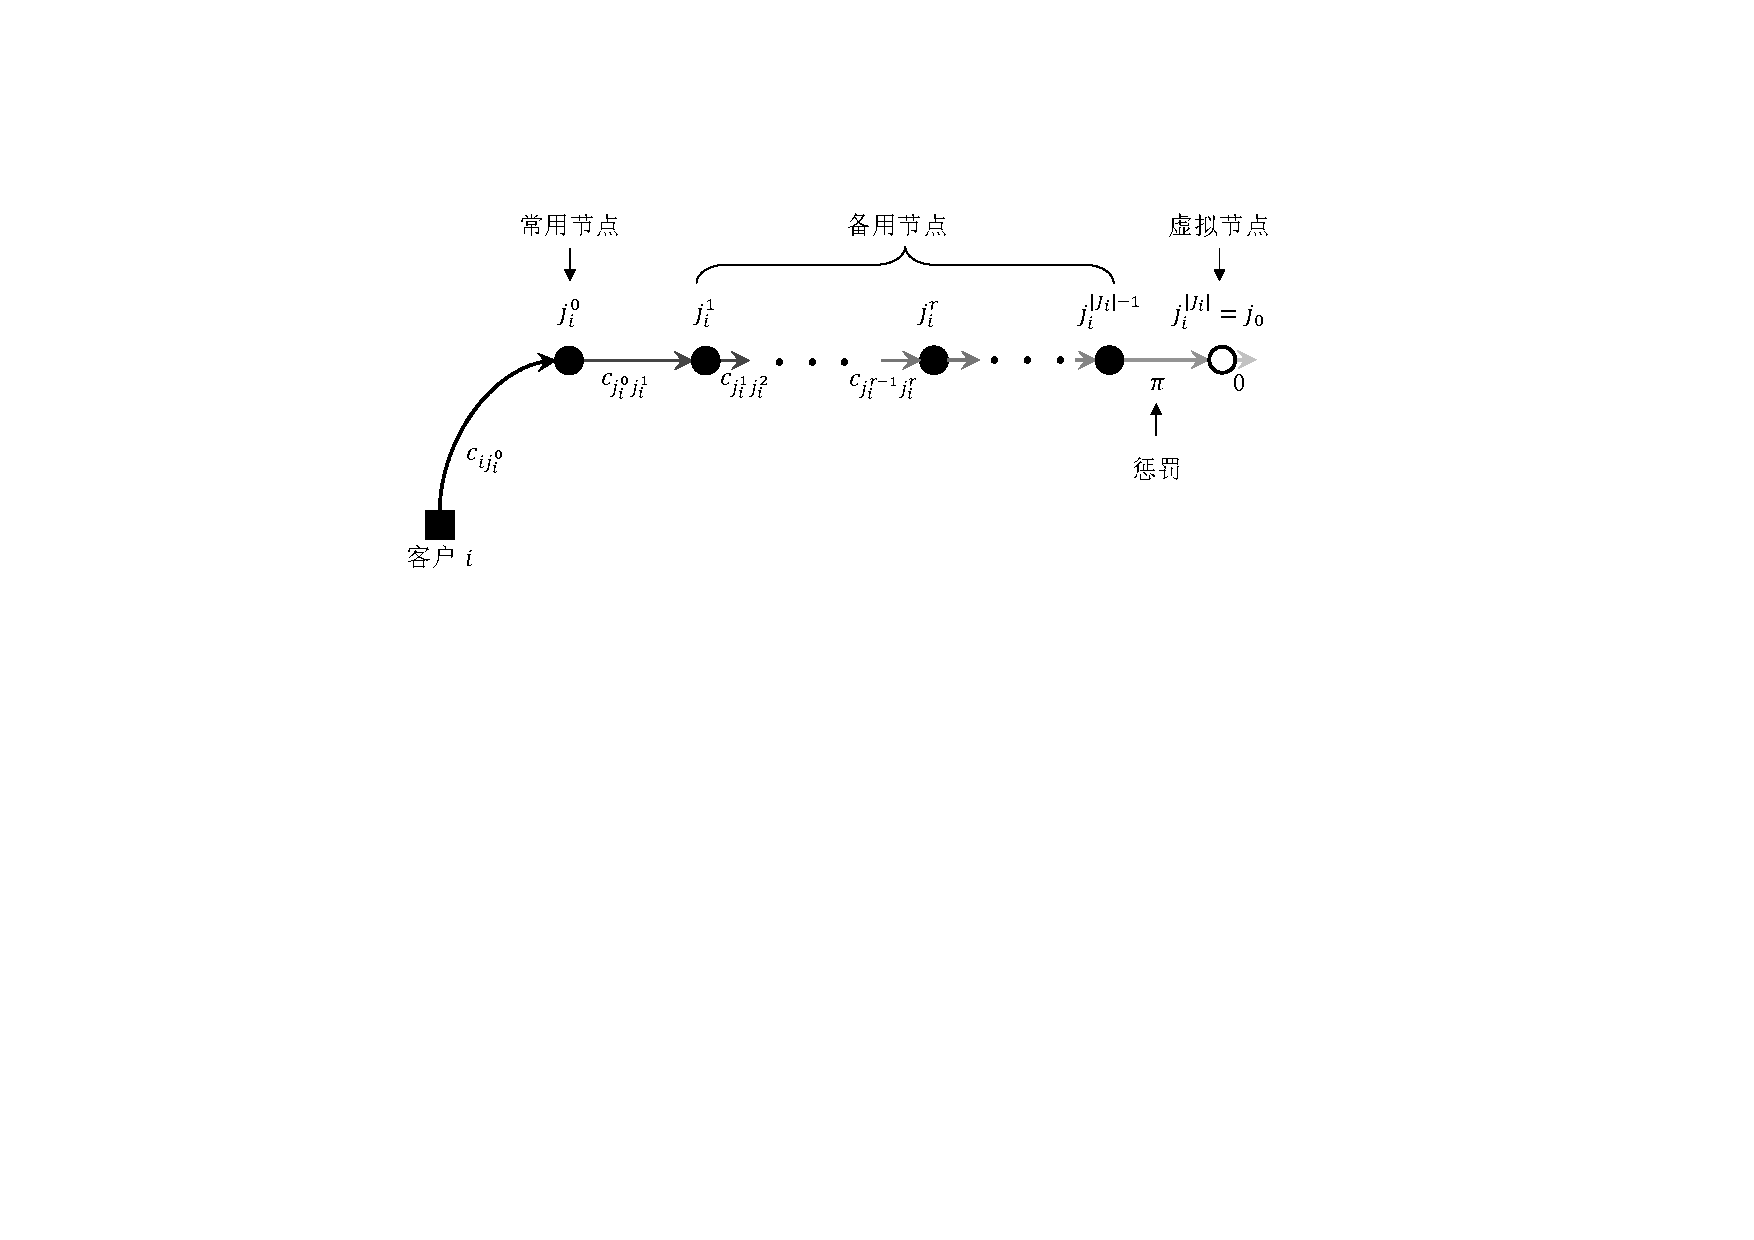
\includegraphics[width=\textwidth
    % height=\dimexpr\pagegoal-\pagetotal-4\baselineskip\relax, % 塞进本页的最后
  ]{figures/试错策略示意图.pdf}
  \caption{客户试错策略示意图\\Fig~\ref{fig:trail}~ A Trail-and-error Strategy of a Customer}
  \label{fig:trail}
\end{figure}

当客户$i$访问节点$j_i^0$时,$j_i^0$以$q_{j_i^0}$的概率失效,
以$1-q_{j_i^0}$的概率提供服务。
如果节点$j_i^0$正常服务,
那么客户$i$从节点$j_i^0$获得服务的期望成本等于$\lambda_i c_{ij_i^0} (1-q_{j_i^0})$。
如果节点$j_i^0$失效,那么客户$i$将从$j_i^0$继续出发访问节点$j_i^1$。
同样,若节点$j_i^1$正常服务,
那么客户$i$从节点$j_i^1$获得服务的期望成本等于$\lambda_i (c_{ij_i^0}+c_{j_i^0j_i^1}) q_i^0(1-q_{j_i^1})$,
即在上一个点$j_i^0$失效的情况下点$j_i^1$没有失效。
若节点$j_i^1$失效,则客户$i$将从$j_i^1$继续出发访问节点$j_i^2$,
以此类推,直至客户接受服务或访问完所有节点。

归纳上述推导过程,客户$i$访问第$r(r\ge 1)$等级的节点的期望成本$C_e^{ir}$,
如公式(\ref{eq:expectcost})所示:
\begin{equation}
\label{eq:expectcost}
C_e^{ir}=\lambda_i 
\left( 
c_{ij_i^0}+ \sum_{m=1}^r c_{j_i^{m-1} j_i^{m}}
\right)
\left( 
\prod_{n=0}^{r-1} q_{j_i^n}-\prod_{n=0}^{r} q_{j_i^n}
\right)
\end{equation}
于是,对所有等级$r$求和,
客户$i$的总期望成本$C_t^i$如公式(\ref{eq:sumcost})所示:
\begin{equation}
\label{eq:sumcost}
C_t^i = \lambda_i \sum_{r=1}^R
\left( 
(c_{ij_i^0}+ \sum_{m=1}^r c_{j_i^{m-1} j_i^{m}})
(\prod_{n=0}^{r-1} q_{j_i^n}-\prod_{n=0}^{r} q_{j_i^n})
\right) +
\lambda_i c_{ij_i^0} (1-q_{j_i^0})
\end{equation}
公式(\ref{eq:sumcost})等号右侧的第一项表示从$r=1$至$r=R$的期望运输成本之和,
右侧第二项表示虚拟节点的期望惩罚成本。
提取前面的一个求和项$r=1$与后面的项合并得到,
\begin{equation}
\begin{aligned}
C_t^i &= \lambda_i \sum_{r=2}^R
\left( 
(c_{ij_i^0}+ \sum_{m=1}^r c_{j_i^{m-1} j_i^{m}})
(\prod_{n=0}^{r-1} q_{j_i^n}-\prod_{n=0}^{r} q_{j_i^n})
\right) \\
& - \lambda_i(\prod_{n=0}^1 q_{j_i^n})(c_{ij_i^0} + \sum_{m=1}^1 c_{j_i^{m-1}j_i^m})\\
& + \lambda_i(c_{ij_i^0} + c_{j_i^{0}j_i^{1}} \prod_{n=0}^0q_{j_i^n})
\end{aligned}
\end{equation}
再提取一项$r=2$与后面的项合并,得到,
\begin{equation}
\begin{aligned}
C_t^i &= \lambda_i \sum_{r=3}^R
\left( 
(c_{ij_i^0}+ \sum_{m=1}^r c_{j_i^{m-1} j_i^{m}})
(\prod_{n=0}^{r-1} q_{j_i^n}-\prod_{n=0}^{r} q_{j_i^n})
\right) \\
& - \lambda_i(\prod_{n=0}^2 q_{j_i^n})(c_{ij_i^0} + \sum_{m=1}^2 c_{j_i^{m-1}j_i^m})\\
& + \lambda_i(c_{ij_i^0} + c_{j_i^{0}j_i^{1}} \prod_{n=0}^0q_{j_i^n} + c_{j_i^{1}j_i^{2}} \prod_{n=0}^1q_{j_i^n})
\end{aligned}
\end{equation}
如此进行,直至全部展开,最终得到,
\begin{equation}
\label{eq:sumcostlast}
\begin{aligned}
C_t^i &= - \lambda_i(\prod_{n=0}^{R} q_{j_i^n})(c_{ij_i^0} + \sum_{m=1}^{R} c_{j_i^{m-1}j_i^m})\\
& + \lambda_i(c_{ij_i^0} + c_{j_i^{0}j_i^{1}} \prod_{n=0}^0q_{j_i^n} + 
 c_{j_i^{1}j_i^{2}} \prod_{n=0}^1q_{j_i^n} + ...
+ c_{j_i^{R-1}j_i^{R}} \prod_{n=0}^{R-1}q_{j_i^n})
\end{aligned}
\end{equation}
由于设定$r=R$时,备用节点一定为虚拟节点,
于是有$q_{j_i^R} = q_{j_0} = 0$,
所以公式(\ref{eq:sumcostlast})的负数项可消除($\prod_{n=0}^{R} q_{j_i^n}=0$),
后面的正数项经过整理,可表示为,
\begin{equation}
\label{eq:sumcostabbr}
C_t^i = \lambda_i
\left( 
    c_{ij_{i}^0} + \sum_{r=1}^R c_{j_i^{r-1}j_i^{r}}(\prod_{n=0}^{r-1} q_{j_i^n})
\right)
\end{equation}
公式(\ref{eq:sumcostabbr})得到了一个客户$i\in I$的期望运输成本,
所有客户的期望运输成本等于:
\begin{equation}
C_t = \sum_{i\in I}\lambda_i
\left( 
    c_{ij_{i}^0} + \sum_{r=1}^R c_{j_i^{r-1}j_i^{r}}(\prod_{n=0}^{r-1} q_{j_i^n})
\right)
\end{equation}

至此,关于客户的期望运输成本的推导已完成。
考虑节点失效风险的物流网络选址问题可正式定义为:
给定一个客户集$I$和节点候选拓展集$\bar{J}$,
以及弧的权重$\{c_{ij}|\forall i \in I\cup \bar{J},\forall j\in \bar{J}\}$,
节点的损坏概率$q_j,\forall j\in \bar{J}$、建设成本$f_j,\forall j\in \bar{J}$,
客户的需求$\lambda_i,\forall i \in I$,
求一个子集$J^*\subseteq \bar{J}$以及每个客户$i$访问子集$J_i^*\subseteq J^*$的序列$s_i = (j_i^0,...,j_i^r,...,j_i^R),\forall j_i^r \in J_i^*,\forall i\in I, r=0,...,R$,
使得建设节点的固定成本$C_f=\sum_{j\in J^*}f_j$与客户的期望运输成本$C_t=\sum_{i\in I}\lambda_i
\left( c_{ij_{i}^0} + \sum_{r=1}^R c_{j_i^{r-1}j_i^{r}}(\prod_{n=0}^{r-1} q_{j_i^n})\right)$之和最小。

最后,建模过程用到的所有符号定义如表\ref{table:符号}所示:

\begin{table}[!htb]\normalsize   %%\small是为了设置表格中的字体比正文小
\setlength{\abovecaptionskip}{-0.05cm} %调整图片caption与正文之间的间距,table同理。可自己调整。
\setlength{\belowcaptionskip}{-0.2cm} 
  \centering
  \renewcommand\arraystretch{1}
  \caption{符号释义表\\Table~\ref{table:符号}~Notation List}
\begin{tabular}{p{1.5cm}<{\centering} l}
 % \begin{tabular}{c}{l}
  \toprule
  \textbf{符号} & \textbf{解释} \\
  \midrule %[2pt]
    $G$   &  有向图      \\
    $V$   &  图$G$的点集      \\
    $A$   &  图$G$的弧集      \\
    $I$   &  客户点集 \\
    $J$   &  候选点集 \\
    $\lambda_i$ & 客户$i\in I$的需求 \\ 
    $f_j$   &  节点$j\in J$的建设成本 \\
    $q_j$   &  节点$j\in J$的失效概率 \\
    $c_{ij}$ & 弧$(i,j)$的权重 \\
    $\pi$ & 惩罚价格 \\
    $j_0$ & 虚拟节点 \\
    $R$ & 每个客户备用节点的最大个数 \\
    $\bar{J}$ & 集合$J$与\{$j_0$\}的并集 \\
    $r$ & 备用节点的等级 \\
    $j_i^r$ & 客户$i$的第$r$等级的节点 \\
    $C_e^{ir}$ & 客户$i$访问第$r$等级备用节点的期望成本 \\
    $C_t^i$ & 客户$i$的总期望运输成本 \\
    $C_t$   & 总期望运输成本 \\
    $C_f$   & 总建设成本 \\
    $J_j^+$ & 可在$j$之前访问的节点集合\\
    $J_j^-$ & 可在$j$之后访问的节点集合\\
    % $y_j$    & 决策变量,决定是否建设节点\\
    % $z_{ij}$ & 决策变量,决定客户的常用节点\\
    % $x_{ijj'r}$ & 决策变量,客户的试错策略\\
    % $p_{ijj'r}$ & 中间变量,记录概率关系\\
    % $w_{ijj'r}$ & 辅助变量,线性化目标函数和约束\\
  \bottomrule
  \end{tabular}
  \label{table:符号}
\end{table}

\section{模型构建}
\label{sec:model}
本节将构建考虑节点失效风险的物流网络选址问题的非线性混合整数规划模型,
该模型的目标函数为最小化总成本,
包括建设节点的固定成本(投资成本)和客户的期望运输成本,
其中期望运输成本的计算过程已在\ref{sec:description}节推导。
第\ref{subsec:obj}节明确了模型的目标函数,
第\ref{subsec:st}节描述了模型的约束。

\subsection{目标函数推导}
\label{subsec:obj}
本小节将构建模型的目标函数,
关于问题描述中符号的定义参见表\ref{table:符号}。
在定义决策变量之前,
为了表达客户访问节点的先后顺序,
本章将采用两点之间是否存在弧的方法表示客户的试错方案。
使用这种``弧''的概念借鉴了车辆路径问题(Vehicle Routing Problem, VRP)的决策变量处理思路\cite{vigo}
以及Albareda等人\cite{rpmp}研究可靠P-中值问题对决策变量的处理。

由于每个客户从自身位置出发,因而起点不同。
定义集合$J_{ij}^+$和集合$J_{ij}^-$分别表示客户$i$在点$j$之前和之后可访问的点集,
\added[id=yrf]{公式如下:}
\begin{equation}
    J_{ij}^+ =
    \begin{cases}
        \{i\} \cup J \backslash \{j\} & \text{ if } j \ne j_0\\
        \{i\} \cup J                  & \text{ if } j = j_0
    \end{cases},
    \forall i \in I, j\in J
    \label{eq:after}
\end{equation}

\begin{equation}
J_{ij}^- =
\begin{cases}
\bar{J} \backslash \{j\} & \text{ if } j \ne i\\
\bar{J}                  & \text{ if } j = i
\end{cases},
\forall i \in I, j\in J
\label{eq:before}
\end{equation}

上述公式(\ref{eq:after})和公式(\ref{eq:before})可解释为:
对于客户$i$,只能从客户点$i$以及不包括节点$j$自身的任意实体节点访问节点$j$,
但可从客户点$i$以及任意实体节点访问虚拟节点$j_0$。
同理,对于客户$i$,客户从$i$出发后可以访问任意节点,
但是访问节点$j$之后访问的下一个点不能再是节点$j$。

该模型共需要两种决策变量和一种中间变量,
具体定义如下:
\begin{enumerate}[label=(\arabic*),leftmargin=0pt,itemindent=3.5\ccwd, nosep]
\item $y_j,\forall j \in J$:
选址0-1决策变量,等于1表示在候选节点$j\in J$处建设节点,
等于0表示不在该处建设。

\item $x_{ijk},\forall i \in I, j \in J\cup \{i\}, k\in J_{ij}^-$:
试错序列0-1决策变量,等于1表示弧$(j,k)$属于客户$i$,
等于0表示弧$(j,k)$不属于客户$i$。

\item $p_{ijk},\forall i \in I, j \in J\cup \{i\}, k\in J_{ij}^-$:
概率连续中间变量,上界等于1下界等于0,
表示客户$i$从节点$j$访问节点$k$的概率。
\end{enumerate}

模型的目标函数是最小化总成本,
包含建设节点的固定成本以及期望运营成本,
具体如公式(\ref{eq:obj})所示。
\begin{equation}
\label{eq:obj}
\min C = \sum_{j\in J}f_jy_j
+ \sum_{i\in I}\lambda_i 
\sum_{k\in J_{ij}^+}\sum_{j\in \bar{J}}
c_{kj} p_{ikj} x_{ikj}
\end{equation}

公式(\ref{eq:obj})的
第一部分计算了建设节点的成本,第二部分计算了期望运输成本。
目标函数中期望运输成本是在公式(\ref{eq:sumcostabbr})的基础上引入决策变量构成的。
公式(\ref{eq:sumcostabbr})的累乘项$\prod_{n=0}^{r-1} q_{j_i^n}$被中间变量$p_{ikj}$替换。
关于$p_{ikj}$的递推关系,
详见约束(\ref{eq:st_probinit})和约束(\ref{eq:st_probmiddle})。
值得注意的是决策变量$x_{ikj}$和中间变量$p_{ikj}$相乘,
因此该目标函数是非线性(二次)的。

\subsection{数学模型}
\label{subsec:st}
考虑节点失效风险的物流网络选址模型如下:
\begin{equation}
\label{eq:obj_model}
\min C = \sum_{j\in J}f_jy_j + \sum_{i\in I}\lambda_i \sum_{k\in J_{ij}^+}\sum_{j\in \bar{J}} c_{kj} p_{ikj} x_{ikj}
\end{equation}
\textit{s.t.}
\begin{gather}
% 指定给开启的节点
\sum_{k\in J_{ij}^+}x_{ikj} \le y_j ,\forall i \in I , j\in J \label{eq:st_assign2open}\\
% 流开始与结束
\sum_{j\in J_{ii}^-}x_{iij} = \sum_{j\in J_{i{j_{0}}}^+} x_{ijj_0} = 1, \forall i \in I  \label{eq:st_flow}\\
% 流平衡
\sum_{k\in J_{ij}^-} x_{ijk} = \sum_{k\in J_{ij}^+} x_{ikj}, \forall i \in I, j \in J \label{eq:st_flowbalance}\\
% 概率初始化
p_{iij} = x_{iij}, \forall i\in I, j\in J_{ii}^- \label{eq:st_probinit}\\
% 概率递推
q_j\sum_{k\in J_{ij}^+} x_{ikj} p_{ikj}= p_{ijj'}, \forall i \in I, j \in J, j'\in J_{ij}^- \label{eq:st_probmiddle} \\
% 尝试次数
\sum_{j\in J\cup\{i\}} \sum_{k\in J_{ij}^-} x_{ijk} \le R, \forall i\in I \label{eq:st_trytimes} \\
% y决策
y_{j} \in\{0,1\}, \forall j \in {J} \label{eq:st_y}\\
% x决策
x_{ijk} \in \{0,1\}, \forall i \in I, j \in J\cup \{i\}, k\in J_{ij}^- \label{eq:st_x}\\
% p决策
0 \le p_{ijk} \le 1, \forall i \in I, j \in J\cup \{i\}, k\in J_{ij}^- \label{eq:st_p}
\end{gather}

目标函数(\ref{eq:obj_model})表示最小化总成本。
约束(\ref{eq:st_assign2open})规定只有已建设的备用节点才有可能成为某个客户的常用或备用节点;
约束(\ref{eq:st_flow})表示客户出发点和终点的流平衡约束,客户必须出发前往某个节点,也必须从某个点到达虚拟节点(终点);
约束(\ref{eq:st_flowbalance})是中间点的流平衡约束,规定进入节点的流量等于流出节点的流量;
约束(\ref{eq:st_probinit})初始化每个客户出发对应弧的概率;
约束(\ref{eq:st_probmiddle})表达了两段相邻弧的概率递推关系;
约束(\ref{eq:st_trytimes})限制了每个客户尝试的次数,即每个客户拥有的弧的个数;
最后,约束(\ref{eq:st_y})和(\ref{eq:st_x})是决策变量0-1整数约束,约束(\ref{eq:st_p})表示中间变量的上下界。

\section{模型线性化}
\label{sec:线性化}
由于第\ref{sec:model}节给出的数学模型是非线性混合整数规划模型,
本小节针对该模型提出了降低模型复杂程度的线性化方法。
模型中的非线性的部分,
分别出现在目标函数(\ref{eq:obj})和约束(\ref{eq:st_probmiddle})中。
采用等价替换方法消除模型中的二次项,
令$w_{ijk} = p_{ijk}x_{ijk},\forall i \in I, j \in J\cup \{i\}, k\in J_{ij}^-$,则目标函数(\ref{eq:obj_model})可替换为,
\begin{equation}
\min C = \sum_{j\in J}f_jy_j + \sum_{i\in I}\lambda_i \sum_{k\in J_{ij}^+}\sum_{j\in \bar{J}} c_{kj} w_{ikj}
\end{equation}
使用相同的方式,替换约束(\ref{eq:st_probmiddle})中的非线性部分,
则约束(\ref{eq:st_probmiddle})变为,
\begin{equation}
q_j\sum_{k\in J_{ij}^+} w_{ikj}= p_{ijj'}, \forall i \in I, j \in J, j'\in J_{ij}^- \label{eq:l_st_probmiddle} \\
\end{equation}
需注意,当前的替换并不是等价的。
$w_{ijk}, \forall i \in I, j \in J, j'\in J_{ij}^-$作为中间变量,在替换时需补充一些等价约束,这些等价约束限制了中间变量的取值范围,保证替换的等价性。
注意到变量$x_{ijk},\forall i \in I, j \in J, k\in J_{ij}^-$为0-1约束,
变量$p_{ijk},\forall i \in I, j \in J, k\in J_{ij}^-$为[0,1]之间的连续变量。
由于$w_{ijk},\forall i \in I, j \in J, k\in J_{ij}^-$等于对应变量相乘,
那么$w_{ijk}$的上界将取二者的较小值,下界将大于二者之和减1,即等价约束如下:
\begin{gather}
% 上界1
w_{ijk} \le p_{ijk}, \forall i \in I, j \in J \cup \{i\}, j'\in J_{ij}^- \\
% 上界2
w_{ijk} \le x_{ijk}, \forall i \in I, j \in J \cup \{i\}, j'\in J_{ij}^- \\
% 下界
w_{ijk} \ge p_{ijk} + x_{ijk} - 1, \forall i \in I, j \in J \cup \{i\}, j'\in J_{ij}^-\\
% 范围
0 \le w_{ijk} \le 1, \forall i \in I, j \in J \cup \{i\}, j'\in J_{ij}^- \label{eq:st_w}
\end{gather}

% 考虑节点失效风险的物流网络选址模型及算法研究
考虑节点失效风险的物流网络选址模型的线性化版本如下:
\begin{equation}
\label{eq:l_obj_model}
\min C = \sum_{j\in J}f_jy_j + \sum_{i\in I}\lambda_i \sum_{k\in J_{ij}^+}\sum_{j\in \bar{J}} c_{kj} w_{ikj}
\end{equation}
\textit{s.t.}
\begin{center}
    约束(\ref{eq:st_assign2open}) - 约束(\ref{eq:st_probinit}) \\
    约束(\ref{eq:st_trytimes}) - 约束(\ref{eq:st_p}) \\
    约束(\ref{eq:l_st_probmiddle}) - 约束(\ref{eq:st_w})
\end{center}

\section{模型性质}
\label{sec:attribute}
% 考虑节点失效风险的物流网络选址模型及算法研究
本节将对考虑节点失效风险的物流网络选址数学模型进行一系列性质分析。
首先,第\ref{subsec:nph}小节简要说明了复杂度理论,
并证明了该模型的NP-hard性质,
其次,第\ref{subsec:subprob}小节提出了该问题的一个子问题,
在本文中称为试错序列问题,
该问题是基本最短路问题更一般的形式。

\subsection{NP-hard}
\label{subsec:nph}
根据复杂度理论,如果一个问题如果能在多项式时间(Polynomial time)内求解,
那么这个问题归类为P问题(Polynomial Problem)。
如果一个问题可以在多项式时间内验证解的正确性,
那么这个问题是非确定性多项式时间问题
(Nondeterministic Polynomial-time Problem)即NP问题。
其中,``非确定性''是指不知道这个解是怎样获得的,且很有可能是猜测的。

显然,P问题是NP问题的子集,因为在多项式时间内能解决的问题,
一定能在多项式时间内验证解的正确性。
但是P问题是否等于NP问题至今没有准确的结论。

在NP问题中,有一类问题称为NP完全问题或NPC问题
(Nondeterministic Polynomial-time Complete Problem)。
当一个问题是NP问题,且所有的NP问题都能多项式归约至这个问题时,
那么这个问题是NPC问题。
这说明NPC问题可以相互多项式归约转化。
如果NPC问题存在多项式时间解法,
则说明所有的NP问题都能在多项式时间内解决,那么就证明了P=NP问题。
当前研究已为一些NPC问题找到了伪多项式时间
(Pseudo Polynomial-time algorithm)算法(
时间复杂度是问题规模的多项式,空间复杂度是问题规模的非多项式),
这类问题称为弱NPC问题,另一类不存在伪多项式时间算法的NPC问题称为强NPC问题。

当一个问题满足``所有的NP问题都能多项式归约至这个问题''的条件时,
那么这个问题称为NP-hard问题(Nondeterministic Polynomial-time Hard Problem)。
这说明NP-hard问题目前没有多项式时间算法,也说明NPC问题属于NP-hard问题。

在简单介绍完复杂度理论后,
接下来将证明考虑节点失效风险的物流网络选址问题是NP-hard问题。
本节将从集合覆盖问题逐步推导至UFL问题,再推导至本文研究的问题。
集合覆盖问题是指一类经典的组合优化问题,
该问题的决定性版本(即,回答为``是''或``否''的问题,例如有一个问题的解,判断其是否为最优解)
是Karp\cite{karp}定义的经典21个NPC问题之一,
其优化版本(即,找到该问题最优解的优化过程)是NP-hard问题。
集合覆盖问题是指给定一个全集$U$包含$m$个元素,
集合$S$中包含了$n$个集合且这$n$个集合的并集等于$U$,
$S=\{ S_1, S_2, ..., S_n\}, \bigcup_{i = 1,...,n}S_i = U$。
在$S$中寻找一个最小的子集,使该子集的并集等于$U$。
关于引理的证明可参考Garey等人\cite{garey1979computers}
对于NPC问题与复杂度理论的详细论述。
证明集合覆盖问题是NPC问题超过了本文的范畴,
因此本文不再复述其具体的证明过程,而直接将其作为引理使用。

\begin{description}[leftmargin=0pt, topsep=0pt, parsep=0pt]
  \item[引理 1] 集合覆盖问题的决定性版本是NPC问题,优化版本是一个NP-hard问题。
  \item[推论 1] 无容量限制固定费用选址问题(UFL)是NP-hard问题。
  \item[证明 1] 关于UFL问题论述所用的符号直接沿用了第\ref{sec:description}节的定义。
  基于集合覆盖问题的定义(符号同样沿用),
  做一个辅助图$H$,$H$分为左右两个部分。
  对于左部分,若存在一个元素$u\in U$,则左侧增加一个点$h_u$。
  对于右部分,若存在一个子集$S_k \subseteq \{h_1, h_2, ... , h_m\}$,
  则在右侧增加一个点$S_k$,子集数量上限为$n$。
  如果$h_u \in S_k $,则存在一条边$e_{h_uS_k}$。
  图$H$构建完成后,将在该图上进一步考虑一个UFL问题。
  令点集$I:=\{h_1, h_2, ... ,h_m\}$表示客户点,
  点集$J:=\{S_1, S_2,...,S_n\}$表示候选节点。
  令UFL问题中,固定成本为1,即$f_j=1$,
  若边$e_{h_uS_k}$存在,则$c_{h_uS_k}=0$。这样,一个UFL问题变为以最少的节点数($H$中右侧)使得每个客户($h_u$)可以被与之相连的节点($S_k$,且$S_k$包含$h_u$)服务。
  该UFL问题就转换成了一个集合覆盖问题。
  显然,当且仅当集合覆盖问题取最优时,这个特殊的UFL问题取最优。
\end{description}

上述的转换过程,称为多项式归约。
它使得一个UFL问题转换成一个已知的NP-hard问题,
进而证明了UFL问题是一个NP-hard问题。
从UFL问题出发,
可推导考虑节点失效风险的物流网络选址问题是NP-hard问题。

\begin{description}[leftmargin=0pt, topsep=0pt, parsep=0pt]
  \item[推论 2] 考虑节点失效风险的物流网络选址问题是NP-hard问题。
  \item[证明 2] 在第\ref{sec:model}节构建的模型中,
  令R=1,则每个客户只有一个常用节点可以使用,无可用的实体备用节点。
  由于常用节点的失效概率已知,则相关价格的期望值也已知。
  那么该问题退化成一个UFL问题,并且由推论1可知UFL问题是NP-hard问题,
  那么未退化的原问题也是NP-hard问题。
  换句话说,该问题拓展了UFL问题,进而也是NP-hard问题。
  该证明详情可参考Li\cite{qingwei}等人的研究。
\end{description}


\subsection{子问题:试错序列问题}
\label{subsec:subprob}
根据客户的试错策略,
本文提出了考虑节点失效风险的物流网络选址问题的一个子问题,
本文称作试错序列问题,
是指在给定已建成的节点集合$J^*$中,
为每个客户指派一条期望成本最低的试错序列。
研究试错序列问题的解法可以带来两方面的好处。
首先,当求解主问题的启发式算法给出了节点选址方案时,
快速求解试错序列问题可以提升评估方案质量的效率。
其次,假设所有的节点均可用并增加访问节点的一项固定成本时,
该问题则是主问题的拉格朗日松弛形式,
这将在第\ref{cha:LR算法}章中介绍。

该问题的正式定义如下:
给定已建设的节点集合$J^*$,客户集合$I$,虚拟节点$j_0$
以及弧的权重$\{c_{ij}|\forall i \in I\cup J^*,\forall j\in J^*\}$,
节点的损坏概率$q_j,j\in J^*$,
客户的需求$\lambda_i,\forall i \in I$,
每个客户最大尝试次数$R$,
对于每个客户$i\in I$来说,求从$i$出发访问$J^*$中的节点,
并前往$j_0$的总期望运输成本最小的序列,
并且该序列的中虚拟节点和已建设节点的总数不超过$R$。
图\ref{fig:trail}展示了这种试错序列的起点与终点定义,
此外,期望运输成本的计算方法参见公式(\ref{eq:sumcostabbr})。
同样,本节给出试错序列问题一般形式的数学模型,
为了方便表述,
该模型使用的符号继承表\ref{table:符号}的定义。
不失一般性地假设$J^* = J$,即所有的设施均被建设。
给定一个客户点$i\in I$,
定义0-1决策变量$z_{kj}, \forall j \in \bar{J}, \forall k \in J_{ij}^+$
等于1时表示客户$i$经过该弧$(k,j)$,
等于0时表示不经过;
连续[0,1]决策变量$p_{kj}, \forall j \in \bar{J}, \forall k \in J_{ij}^+$
表示客户$i$经过弧$(k,j)$的概率,
试错序列模型如下:

\begin{equation}
\min C^i_t = \lambda_i \sum_{k\in J_{ij}^+}\sum_{j\in \bar{J}} c_{kj} p_{kj} z_{kj} \label{eq:tes_obj}
\end{equation}
\textit{s.t.}
\begin{gather}
% 流开始与结束 trail-error-sequence tes
\sum_{j\in J_{ii}^-}z_{ij} = \sum_{j\in J_{i{j_{0}}}^+} z_{jj_0} = 1 \label{eq:tes_flow}\\
% 流平衡
\sum_{k\in J_{ij}^-} z_{jk} = \sum_{k\in J_{ij}^+} z_{kj}, \forall j \in J \label{eq:tes_flow_balance}\\
% 概率初始化
p_{ij} = z_{ij}, \forall j\in J_{ii}^- \label{eq:tes_probinit} \\
% 概率递推
q_j\sum_{k\in J_{ij}^+} z_{kj} p_{kj}= p_{jj'}, \forall j \in J, j'\in J_{ij}^-  \label{eq:tes_probmiddle}\\
% 尝试次数
\sum_{j\in J\cup\{i\}} \sum_{k\in J_{ij}^-} z_{jk} \le R \label{eq:tes_maxtry}\\
% x决策
z_{jk} \in \{0,1\},  \forall j \in \bar{J}, \forall k \in J_{ij}^+ \label{eq:tes_z}\\
% p决策
0 \le p_{ijk} \le 1, \forall j \in \bar{J}, \forall k \in J_{ij}^+ \label{eq:tes_p}
\end{gather}

模型的目标(\ref{eq:tes_obj})是最小化客户$i$的总期望运输成本;
约束(\ref{eq:tes_flow})和约束(\ref{eq:tes_flow_balance})是流出发、结束和守恒约束;
约束(\ref{eq:tes_probinit})和约束(\ref{eq:tes_probmiddle})是概率初始化和递推关系;
约束(\ref{eq:tes_maxtry})规定客户的试错次数;
约束(\ref{eq:tes_z})和约束(\ref{eq:tes_p})是整数约束和连续变量的上下界约束。
注意第\ref{sec:线性化}节的线性化技术同样适用于求解该问题,
在此不再赘述试错序列模型的线性化版本。

试错序列问题本质上属于最短路问题的变种,
是资源受限的基本最短路问题
(Elementary Shortest Path Problem with Resource Constraints, ESPPRC)的特殊形式。
该\replaced[id=yrf]{特殊形式的ESPPRC}{ESPPRC的特殊形式}的定义如下:
给定一个图$H=(V_H,E_H)$,其中$s\in E_H$是源点,$t\in E_H$是汇点,
每个点$v\in E_H$的需求为$\lambda_v$,每条边$e_H\in E_H$的距离为$c_{e_H}$,
求一条从$s$到$t$的路径,使得该路径的总距离之和最小的同时,
路径上所有经过的点的需求和不超过$Q$。

注意上述定义是ESPPRC问题的特殊形式,仅考虑了容量限制。
事实上,ESPPRC问题中每个点有时间窗限制,
但在本节讨论的问题中并无该限制,
因此做出了简化(可将每个点的时间窗无限放宽以消除时间窗)。
有关ESPPRC详尽的阐述与求解方法,可见参考文献\cite{pulse}。
\added[id=yrf]{
给定一个客户$i\in I$,
令$s=i$,$t=j_0$,$\lambda_v=1$,$c_{e_H}=c_{ij}$,$Q=R$,$q_j=1,\forall j\in J^*$
}
% \deleted{\mobox{令$V^i_H = J^* \cup \{i\}$,$Q=R$,$q_j=1,j\in J^*$}}
则试错序列问题等价于ESPPRC问题。
由于ESPPRC问题已被证明是NP-Hard问题\cite{Dror1994},
进而试错序列问题也是NP-Hard问题。
这说明当前不存在求解该问题的多项式时间算法。

综上,试错序列问题是基本最短路问题的一个变种,
每个节点附加的失效概率和期望目标成本增加了求解的难度。
本文的第\ref{cha:LR算法}章设计的拉格朗日松弛算法在求解上界与下界时,
都不可避免地多次求解这个问题,
求解该问题的算法将在第\ref{subsec:下界获取}节详细阐述。

\section{本章小结}
\label{sec:小结3}
本章的核心内容是构建考虑节点失效风险的物流网络选址模型。
在建立模型之前,使用数学语言的严谨描述了该问题,
并对客户的试错行为进行刻画,推导了由此产生的期望运输成本。
引入决策变量构建了二次约束二次目标的混合整数规划模型,
使用线性化的方法消除了模型中非线性的部分,使得精确求解模型的难度降低。
为了方便后续算法开发,本节\replaced[id=yrf]{研究了}{提出了}客户试错序列子问题,
\added[id=yrf]{开发求解该子问题的有效算法可加速求解主问题的过程。}
\deleted[id=yrf]{解决该子问题的有效方法可加快元启发式算法中评估解的质量的过程}
最后,由于该问题被证明为NP-hard问题,
为了求解大规模算例,
第\ref{cha:LR算法}章开发了基于迭代局部搜索改进的拉格朗日松弛算法。